\section{Протоколы передачи: UART, PWM, PPM, SBUS}

Протоколы нужны, чтобы передавать команды \textbf{от приёмника к полётному контроллеру} и \textbf{от контроллера к регуляторам/сервоприводам}, а также связывать ПК с периферией (GPS, VTX, телеметрия).

\begin{figure}[H]\centering
\begin{tikzpicture}[font=\sffamily\small,node distance=24mm]
\node[blk,fill=blk3] (tx) {Пульт};
\node[blk,fill=blk2,right=of tx] (rx) {Приёмник};
\node[blk,fill=blk1,right=of rx] (fc) {Полётный\\контроллер};
\node[blk,fill=blk4,right=of fc] (esc) {ESC\,/\,сервы};
\draw[arr,decorate,decoration={snake,amplitude=.8mm,segment length=4mm,post length=2mm}] (tx) -- node[above,font=\scriptsize]{радио} (rx);
\draw[arr] (rx) -- node[above,font=\scriptsize]{PWM, PPM,} node[below,font=\scriptsize]{SBUS, CRSF} (fc);
\draw[arr] (fc) -- node[above,font=\scriptsize]{PWM, OneShot,} node[below,font=\scriptsize]{DShot} (esc);
\end{tikzpicture}
\caption{Где какие протоколы используются}
\end{figure}

\subsection{UART — универсальный асинхронный приёмопередатчик}
\begin{itemize}
\item Аппаратный интерфейс микроконтроллера, на котором работает большинство «серийных» протоколов (SBUS, CRSF, IBUS, GPS, MSP, MAVLink, SmartAudio).
\item Линии: \textbf{TX} (передача), \textbf{RX} (приём), \textbf{GND}. Подключение \textbf{крест-накрест}: TX одного устройства $\to$ RX другого. Двусторонний (full duplex).
\item \term{Асинхронный} — нет отдельной линии тактирования, обе стороны заранее договариваются о \term{скорости} (baud rate): 9600, 57600, 115200, 420000 бод\ldots
\item Кадр: в покое линия в «1» $\to$ \textbf{стартовый бит} «0» $\to$ 8 бит данных (младший первым) $\to$ [бит чётности] $\to$ \textbf{стоповый бит(ы)} «1». Формат записывают как \code{8N1} (8 бит, без чётности, 1 стоп) или \code{8E2}.
\end{itemize}

\begin{figure}[H]\centering
\begin{tikzpicture}[x=9mm,y=7mm,font=\sffamily\scriptsize]
\draw[very thick,accent] (0,1) -- (1,1) -- (1,0) -- (2,0) -- (2,1) -- (3,1) -- (3,0) -- (8,0) -- (8,1) -- (9,1) -- (9,0) -- (10,0) -- (10,1) -- (12,1);
\foreach \x in {1,...,11} \draw[gray!50,dashed] (\x,-0.2) -- (\x,1.3);
\node at (0.5,1.5) {покой};
\node at (1.5,1.5) {\textbf{старт}};
\foreach \i/\b in {0/1,1/0,2/0,3/0,4/0,5/0,6/1,7/0} \node at (2.5+\i,1.5) {D\i};
\foreach \i/\b in {0/1,1/0,2/0,3/0,4/0,5/0,6/1,7/0} \node[text=gray] at (2.5+\i,-0.45) {\b};
\node at (10.5,1.5) {\textbf{стоп}};
\node at (11.5,1.5) {покой};
\draw[decorate,decoration={brace,mirror,amplitude=4pt}] (2,-0.8) -- (10,-0.8) node[midway,below=4pt] {байт 0x41 = «A», младший бит первым};
\end{tikzpicture}
\caption{Кадр UART 8N1 для символа «A»}
\end{figure}

\photo{0.45\linewidth}{runcam.jpg}{Подключение устройства к ПК по UART: TX $\to$ RX, RX $\to$ TX, общий GND}{ArduPilot Wiki}

\subsection{PWM — широтно-импульсная модуляция}
\begin{itemize}
\item Самый старый способ: \textbf{один провод на каждый канал}. Значение канала кодируется \textbf{длительностью импульса}: \SI{1000}{\micro\second} — минимум, \SI{1500}{\micro\second} — центр, \SI{2000}{\micro\second} — максимум.
\item Период — \SI{20}{\milli\second} (частота \SI{50}{\hertz}) для аналоговых сервоприводов, до 400--490~Гц для ESC.
\item Минусы: много проводов (8 каналов — 8 сигнальных проводов), медленно, нет телеметрии. Сегодня — только для серв и простых самолётов.
\end{itemize}

\begin{figure}[H]\centering
\begin{tikzpicture}[x=5mm,y=6mm,font=\sffamily\scriptsize]
\draw[->] (0,0) -- (25,0) node[right] {$t$};
\draw[very thick,accent] (0,0) -- (1,0) -- (1,1) -- (2,1) -- (2,0) -- (11,0) -- (11,1) -- (12.5,1) -- (12.5,0) -- (21,0) -- (21,1) -- (23,1) -- (23,0) -- (24,0);
\node[above] at (1.5,1) {1000\,мкс};
\node[above] at (11.75,1) {1500\,мкс};
\node[above] at (22,1) {2000\,мкс};
\node[below] at (1.5,0) {минимум};
\node[below] at (11.75,0) {центр};
\node[below] at (22,0) {максимум};
\draw[<->] (1,-1.1) -- node[below] {период 20\,мс (50\,Гц)} (11,-1.1);
\end{tikzpicture}
\caption{Сигнал PWM: значение задаётся шириной импульса}
\end{figure}

\subsection{PPM (CPPM) — импульсно-позиционная модуляция}
\begin{itemize}
\item \textbf{Все каналы по одному проводу}, друг за другом. Значение канала — \textbf{интервал между соседними импульсами} (\SIrange{1000}{2000}{\micro\second}).
\item После последнего канала — длинная пауза (> \SI{3}{\milli\second}) для синхронизации. Кадр $\approx$ \SI{22.5}{\milli\second}, обычно \textbf{до 8 каналов}.
\item Плюс — один провод. Минусы — мало каналов, большая задержка, чувствительность к джиттеру. Сегодня устарел.
\end{itemize}

\begin{figure}[H]\centering
\begin{tikzpicture}[x=4mm,y=6mm,font=\sffamily\scriptsize]
\draw[->] (0,0) -- (38,0) node[right] {$t$};
\def\p#1{-- (#1,0) -- (#1,1) -- ({#1+0.4},1) -- ({#1+0.4},0)}
\draw[very thick,accent] (0,0) \p{1} \p{4} \p{7.5} \p{10} \p{13.5} \p{16.5} \p{19} \p{22.5} \p{25} -- (35,0) \p{35} -- (37,0);
\foreach \a/\b/\n in {1/4/1,4/7.5/2,7.5/10/3,10/13.5/4,13.5/16.5/5,16.5/19/6,19/22.5/7,22.5/25/8}
  \draw[<->,gray] (\a,1.4) -- node[above,text=black] {CH\n} (\b,1.4);
\draw[<->] (25,-0.6) -- node[below] {синхропауза} (35,-0.6);
\draw[decorate,decoration={brace,mirror,amplitude=4pt}] (1,-1.4) -- (35,-1.4) node[midway,below=4pt] {один кадр $\approx$ 22,5\,мс};
\end{tikzpicture}
\caption{Сигнал PPM: 8 каналов в одном проводе}
\end{figure}

\begin{figure}[H]\centering
\begin{minipage}{0.46\linewidth}\centering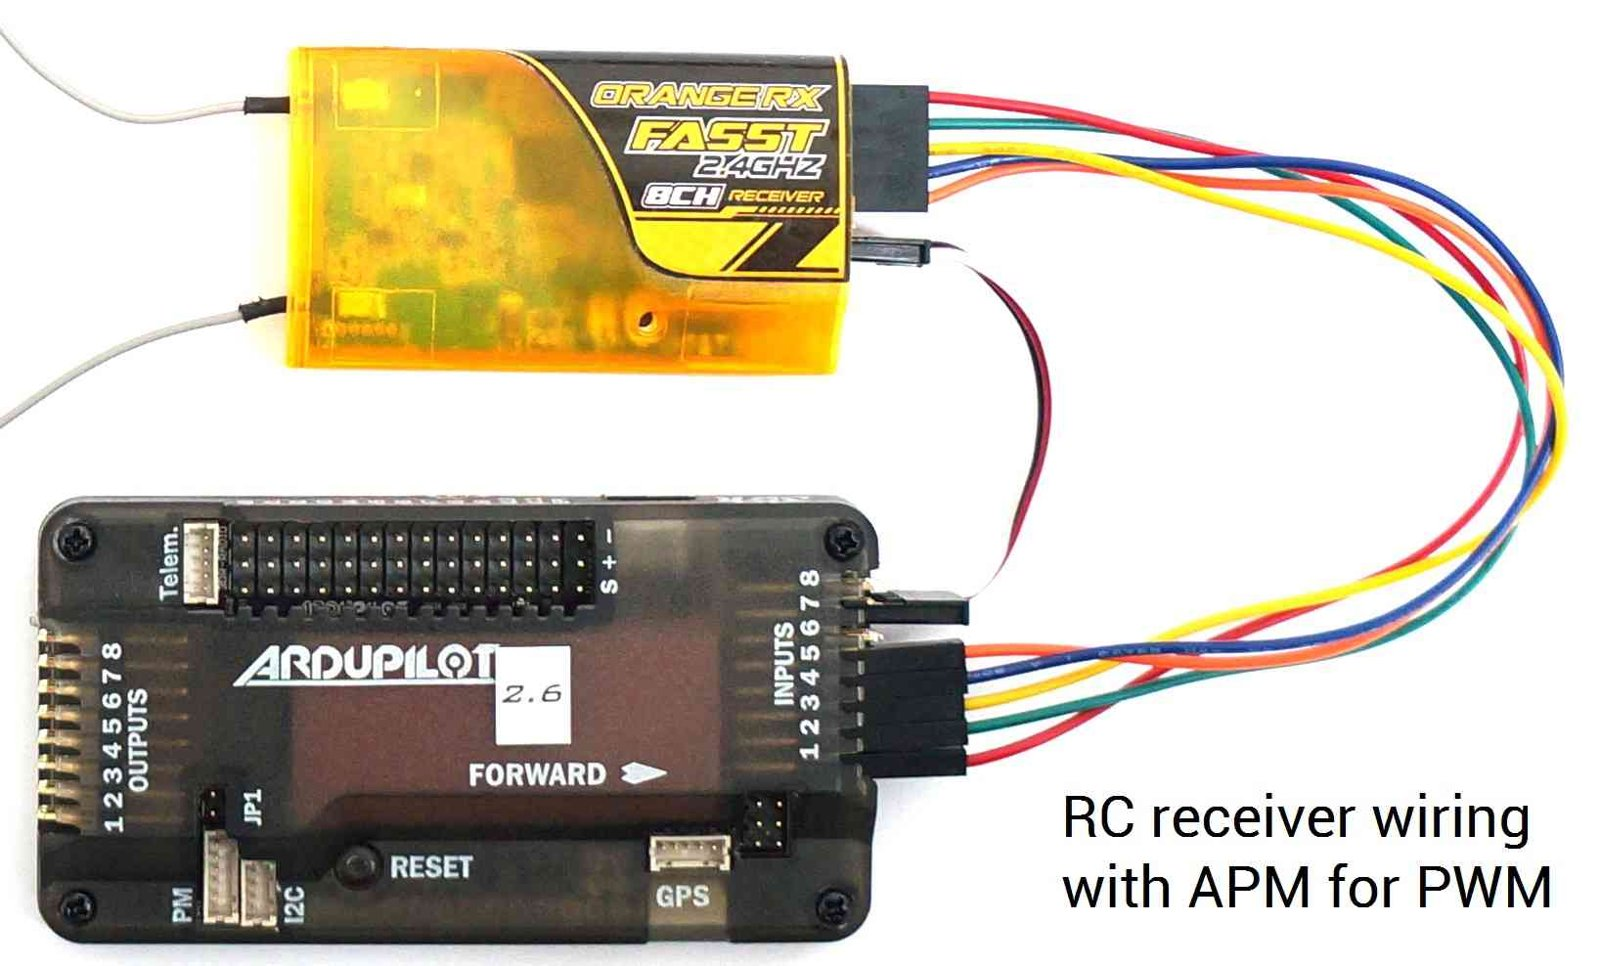
\includegraphics[width=\linewidth]{img/pwm-wiring.jpg}\\{\small PWM: отдельный провод на каждый канал}\end{minipage}\hfill
\begin{minipage}{0.46\linewidth}\centering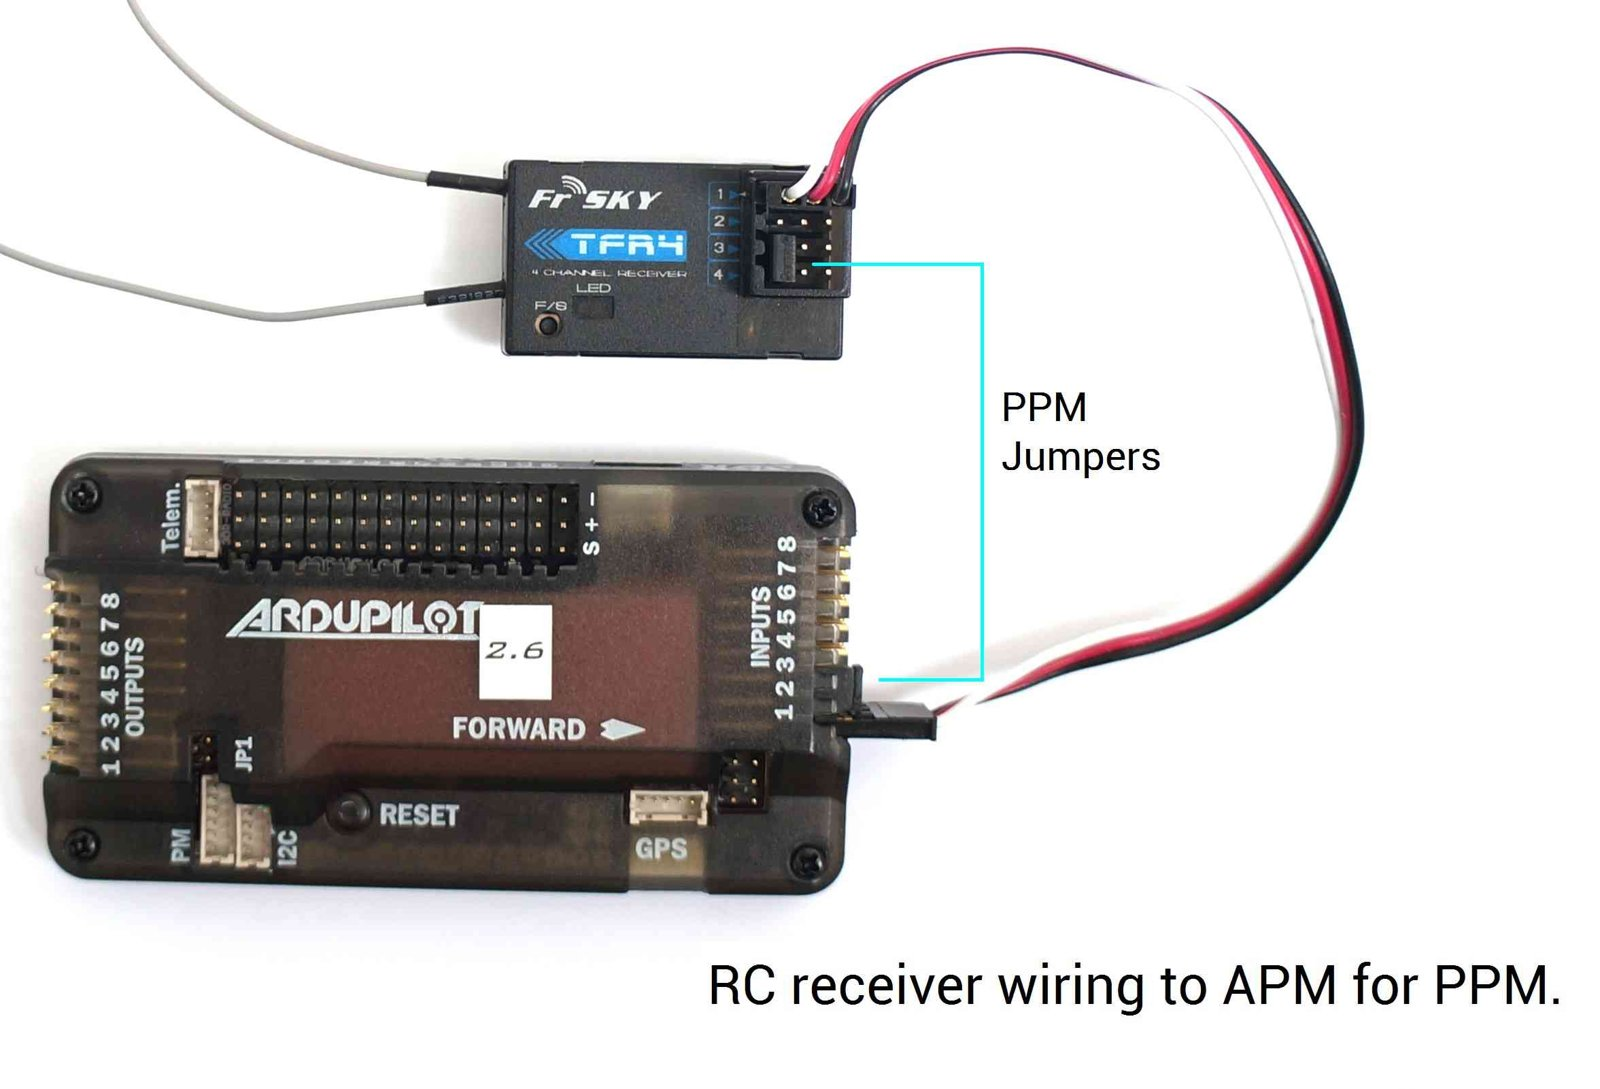
\includegraphics[width=\linewidth]{img/ppm-wiring.jpg}\\{\small PPM: все каналы по одному проводу}\end{minipage}
\caption{Подключение приёмника по PWM и PPM {\color{gray}\scriptsize(фото: ArduPilot Wiki)}}
\end{figure}

\subsection{SBUS (Futaba S.BUS)}
\begin{itemize}
\item \textbf{Цифровой последовательный} протокол поверх UART, разработан Futaba, широко применяется FrSky и другими.
\item Параметры UART: \SI{100000}{бод}, \code{8E2} (чётность even, 2 стоп-бита), \textbf{инвертированный сигнал} — поэтому на F4-контроллерах нужен специальный вход с инвертором (на F7/H7 инверсия есть в самом UART).
\item Кадр \textbf{25 байт}: заголовок \code{0x0F} + 22 байта данных (\textbf{16 каналов по 11 бит}, значения 0–2047) + байт флагов (2 цифровых канала, \textbf{frame lost}, \textbf{failsafe}) + конец \code{0x00}. Кадр каждые \SI{14}{\milli\second} (или 7~мс в быстром режиме).
\item Только в одну сторону. Телеметрию FrSky передаёт отдельно по \textbf{S.Port} или совмещённо в протоколе \textbf{FPort}.
\end{itemize}

\begin{figure}[H]\centering
\begin{tikzpicture}[font=\sffamily\scriptsize,x=5.9mm,y=7mm]
\draw[fill=blk4] (0,0) rectangle (2,1) node[midway] {0x0F};
\draw[fill=blk1] (2,0) rectangle (24,1) node[midway] {22 байта = 16 каналов × 11 бит};
\draw[fill=blk3] (24,0) rectangle (26,1) node[midway] {флаги};
\draw[fill=blk4] (26,0) rectangle (28,1) node[midway] {0x00};
\node[below] at (1,0) {заголовок}; \node[below] at (25,0) {ch17,18, FS}; \node[below] at (27,0) {конец};
\end{tikzpicture}
\caption{Кадр SBUS (25 байт)}
\end{figure}

\subsection{Другие протоколы (полезно знать)}
\begin{table}[H]\centering\small
\renewcommand{\arraystretch}{1.25}
\begin{tabularx}{\linewidth}{@{}p{24mm} X@{}}
\toprule
\textbf{CRSF} & Протокол TBS Crossfire, используется и в \textbf{ELRS}. UART \SI{420000}{бод} \code{8N1}, не инвертирован, до 16 каналов, \textbf{двусторонний}: телеметрия (RSSI, LQ, напряжение, GPS) идёт обратно в пульт. Кадр: \code{[0xC8][длина][тип][данные][CRC8]}. Сейчас — стандарт де-факто. \\
\textbf{IBUS} & FlySky, UART 115200 бод, 32-байтный кадр, 14 каналов. \\
\textbf{FPort} & FrSky: SBUS + S.Port-телеметрия в одном проводе. \\
\textbf{DSM/DSMX} & Spektrum, спутниковые приёмники по UART. \\
\textbf{MSP} & MultiWii Serial Protocol — обмен ПК с конфигуратором, OSD в цифровых очках (MSP DisplayPort), VTX. \\
\textbf{MAVLink} & Телеметрия и команды ArduPilot/PX4 $\leftrightarrow$ наземная станция. \\
\textbf{I$^2$C, SPI, CAN} & Внутренние шины: SPI — гироскоп, OSD, флеш; I$^2$C — компас, барометр, дисплей; CAN (DroneCAN) — GPS, ESC, датчики на ArduPilot. \\
\bottomrule
\end{tabularx}
\caption{Другие протоколы связи}
\end{table}

\subsection{Протоколы ПК $\to$ ESC}
\begin{table}[H]\centering\small
\begin{tabular}{@{}llll@{}}
\toprule
\textbf{Протокол} & \textbf{Тип} & \textbf{Длительность / скорость} & \textbf{Особенность} \\
\midrule
PWM & аналоговый & 1000–2000 мкс & нужна калибровка ESC \\
OneShot125 & аналоговый & 125–250 мкс & в 8 раз быстрее PWM \\
OneShot42 / MultiShot & аналоговый & 42–84 / 5–25 мкс & ещё быстрее \\
\textbf{DShot150/300/600} & \textbf{цифровой} & 150/300/600 кбит/с & без калибровки, CRC, команды \\
Bidirectional DShot & цифровой & — & обратно — обороты (RPM-фильтр) \\
\bottomrule
\end{tabular}
\caption{Протоколы управления регуляторами}
\end{table}
\textbf{Кадр DShot — 16 бит}: 11 бит газа (0 — стоп, 1–47 — команды, 48–2047 — газ), 1 бит запроса телеметрии, 4 бита контрольной суммы. «1» и «0» различаются длительностью высокого уровня внутри бита.

\begin{exam}
\begin{enumerate}
\item Как в PWM кодируется значение канала? А в PPM?
\item Сколько каналов у SBUS, какова скорость и почему на F4 нужен инвертор?
\item Как подключается UART-устройство к ПК? Что означает запись 8N1?
\item Чем DShot лучше PWM для управления моторами?
\end{enumerate}
\end{exam}
